\documentclass[12pt]{report}
\usepackage{graphicx}
\usepackage{titling}
\usepackage{fancyhdr}
\usepackage[latin1]{inputenc}
\usepackage{enumerate}
\usepackage{float}
\usepackage{latexsym}
\usepackage{amssymb}
\usepackage{amsthm}
\usepackage{amsfonts}
\usepackage[usenames,dvipsnames,svgnames,table]{xcolor}
\usepackage{listings}
\usepackage[hidelinks]{hyperref}
\parindent=0pt
\frenchspacing

\pagestyle{fancy}

\fancyhead[L]{\slshape\footnotesize December 3, 2014\\\textsc{02515 Health Care Technology}}
\fancyhead[R]{\slshape\footnotesize \textsc{Andreas Kjeldsen (s092638)}\\\textsc{Morten Eskesen (s133304)}}
\fancyfoot[C]{\thepage}

\newcommand{\tab}{\hspace*{2em}}
\newcommand{\HRule}{\rule{\linewidth}{0.5mm}}

\begin{document}

\begin{titlepage}
\begin{center}


\includegraphics[scale=2.0]{../GFX/dtu_logo.pdf}\\[1cm]

\textsc{\LARGE Technical University of Denmark}\\[1.5cm]

\textsc{\Large 02515 Health Care Technology}\\[0.5cm]


% Title
\HRule \\[0.4cm]
{\huge \bfseries Training Memory Game}\\[0.1cm]
\HRule \\[1.5cm]

% Author and supervisor
\large
\emph{Authors:}
\\[10pt]
Andreas Hallberg \textsc{Kjeldsen}\\
\emph{s092638@student.dtu.dk}
\\[10pt]
Morten Chabert \textsc{Eskesen}\\
\emph{s133304@student.dtu.dk}

\vfill

% Bottom of the page
{\large December 3, 2014}

\end{center}
\end{titlepage}

\chapter{Introduction}
\section{Formalities}
This report is a result of a project done in the course \emph{Health Care Technology} taken at DTU. The project has been a collaboration between us both, Andreas and Morten, where we each have been equally responsible for all parts of the project. Andreas' mother works at an elementary school and by virtue of that we were able to test the game on kids from elementary school. 

\section{Objectives}
The objective and product of the course Health Care Technology is to create a health-promoting interactive game by using Unity and Kinect technology. The game should solve a health care problem in Denmark. The course puts a lot of focus on health care challenges in today's Denmark and how the challenges can be solved by modern technology. In the future we will rely more and more on modern technology for health care problem as one of the problems in health care is the increasing need for treatment of the aging population. Another problem is the number of obese people in Denmark which has increased considerably in the last decade \cite{Sundhedsstyrelsen}.\\
This project aims to aid the solving of the increasing obesity problem in Denmark by creating a game that will increase the physical activity of children such that obesity can be prevented and obese children can become more healthy.

\section{Overweight \& obesity}
Overweight and obesity are defined as abnormal or excessive fat accumulation that presents a risk to health \cite{who-obesity}. An international measure known as Body Mass Index, henceforth \emph{BMI}, is commonly used to classify people as underweight, overweight and obese. BMI values are age-independent and the same for both sexes \cite{who-bmi}. BMI is calculated by the following:

\begin{center}
BMI $=$ $\frac{Weight (kg)}{Height (m)^2}$
\end{center}
When calculating this you can use it to see if you are classified as underweight, normal, overweight or obese by the BMI scale. The BMI classifications and their corresponding values are defined as follows \cite{who-bmi}:
\begin{center}
\begin{tabular}{| c | c | c | c}
\hline
Classification & BMI\\ \hline
Underweight & Below 18.5 \\ \hline
Normal range & 18.5 - 24.99 \\ \hline
Overweight & Over 25\\ \hline
Obese & Over 30 \\ \hline
\end{tabular}
\end{center}
Overweight and obesity are major risk factors for a number of chronic diseases. These diseases include diabetes, cardiovascular diseases and cancer. In Denmark the total expenses linked with obesity and the treatment thereof on hospital was calculated as being 1.1 billion kroner in 2004 \cite{consequences-obese}.

\chapter{Game details}
\section{Requirements specification}


\section{Game description}


\section{Technology}


\section{Game specification}


\chapter{Implementation}


\section{Implementation order}


\chapter{Test}
\section{Test specification}


\section{Test results}
Our game was tested on kids in age range 12-15 at an elementary school in Helsing\o r. The game was therefore tested in an environment with furniture in the background, where the furniture had no effect on the registration of joints. One of the measurable features of a training game is the heart rate of the player. When testing we noted the heart rate of the player before and after playing the game. What follows is a table of the test results obtaining from the elementary school.

Players occurring with the same name are not different players but the same player's second try. HR is Heart Rate, the first number is the before heart rate and the second number is the heart rate after - i.e. 76 $\rightarrow$ 114 means a heart rate of 76 before and 114 after playing. The percentage describes how much the heart rate increased in percentage. FR is Failure Reason where the following codes apply:
\begin{itemize}
\item[1] Wrong exercise done by the player
\item[2] Time ran out, i.e. no exercise was done in time
\item[3] Registration error
\item[4] Computer crashed
\end{itemize}

\begin{center}
\begin{tabular}{ | c | c | c | c | c | c | c | c | c | c |}
\hline
Name & Age & Gender & HR & Diff. & \% & Round & Score & FR\\ \hline
Amine & 15 & F & 76 $\rightarrow$ 114 & 38 & 50 & 5 & 2264 & 1\\ \hline 
Anders & 15 & M & 64 $\rightarrow$ 93 &  29 & 45.3 & 3 & 253 & 1\\ \hline 
Anders & 15 & M & 67 $\rightarrow$ 102  & 35 & 52.2  & 4 & 1057 & 1\\ \hline 
%Andreas & 24 & M & 72 $\rightarrow$ 163 &  & y & 17 & 86505 & \\ \hline 
Ditte & 14 & F & 69 $\rightarrow$ 117 & 48  & 70 & 9 & 10045 & 4\\ \hline 
Ditte & 14 & F & 74 $\rightarrow$ 141 & 67 & 90.5 & 12 & 27497 & 1\\ \hline 
Frederik & 15 & M & 73 $\rightarrow$ 94 & 21 & 28.8 & 3 & 342 & 2\\ \hline 
Freja & 13 & F & 72 $\rightarrow$ 80 &  8 & 11.1 & 2 & 58 & 1\\ \hline 
Freja & 13 & F & 77 $\rightarrow$ 96 &  19 & 24.7 & 3 & 143 & 3\\ \hline 
Imon & 15 & M & 78 $\rightarrow$ 100 & 22 & 28.2 & 5 & 1971 & 1\\ \hline 
Isabella & 15 & F & 73 $\rightarrow$ 120 & 47 & 64.4 & 7 & 6132 & 1\\ \hline 
Jasper & 15 & M & 71 $\rightarrow$ 87  & 16 & 22.5 & 3 & 652 & 1\\ \hline 
Jasper & 15 & M & 73 $\rightarrow$ 123 & 50 & 68.5 & 7 & 6129 & 1\\ \hline 
L\ae rke & 12 & F & 79 $\rightarrow$ 106 & 27 & 34.2 & 4 & 1077 & 3\\ \hline 
L\ae rke & 12 & F & 73 $\rightarrow$ 121 & 48 & 65.8 & 11 & 18528 & 1\\ \hline 
Marcus & 12 & M & 76 $\rightarrow$ 114 & 41 & 54 & 4 & 3308 & 1\\ \hline 
Marcus & 12 & M & 73 $\rightarrow$ 132 & 59 & 80.8 & 13 & 36939 & 1\\ \hline 
Nicklas & 15 & M & 64 $\rightarrow$ 104 & 40 & 62.5 & 5 & 1983 & 1\\ \hline 
Nicklas & 15 & M & 73 $\rightarrow$ 114 & 41 & 56.2 & 8 & 6931 & 1\\ \hline 
Philip & 13 & M & 73 $\rightarrow$ 127 & 54 & 74 & 9 & 10116 & 1\\ \hline 
Philip & 13 & M & 78 $\rightarrow$ 141 & 63 & 80.8 &12 & 22991& 1\\ \hline 
Siw & 15 & F & 74 $\rightarrow$ 123 & 49 & 66.2 & 5 & 1411 & 2\\ \hline 
Siw & 15 & F & 72 $\rightarrow$ 129 & 57 & 79.2 & 12 & 19345 & 1\\ \hline 
Zenah & 13 & F & 74 $\rightarrow$ 91 & 17 & 23 & 4 & 1304 & 1\\ \hline 
Zenah & 13 & F & 83 $\rightarrow$ 112 & 29 & 34.9 & 8 & 9775 & 1\\ \hline
Average & 13.9 & \multicolumn{2}{r}{} & & 52.9 & 6.9 & 7927.1 & \\ \hline
\end{tabular}
\end{center}

\begin{figure}[H]
	\centering
	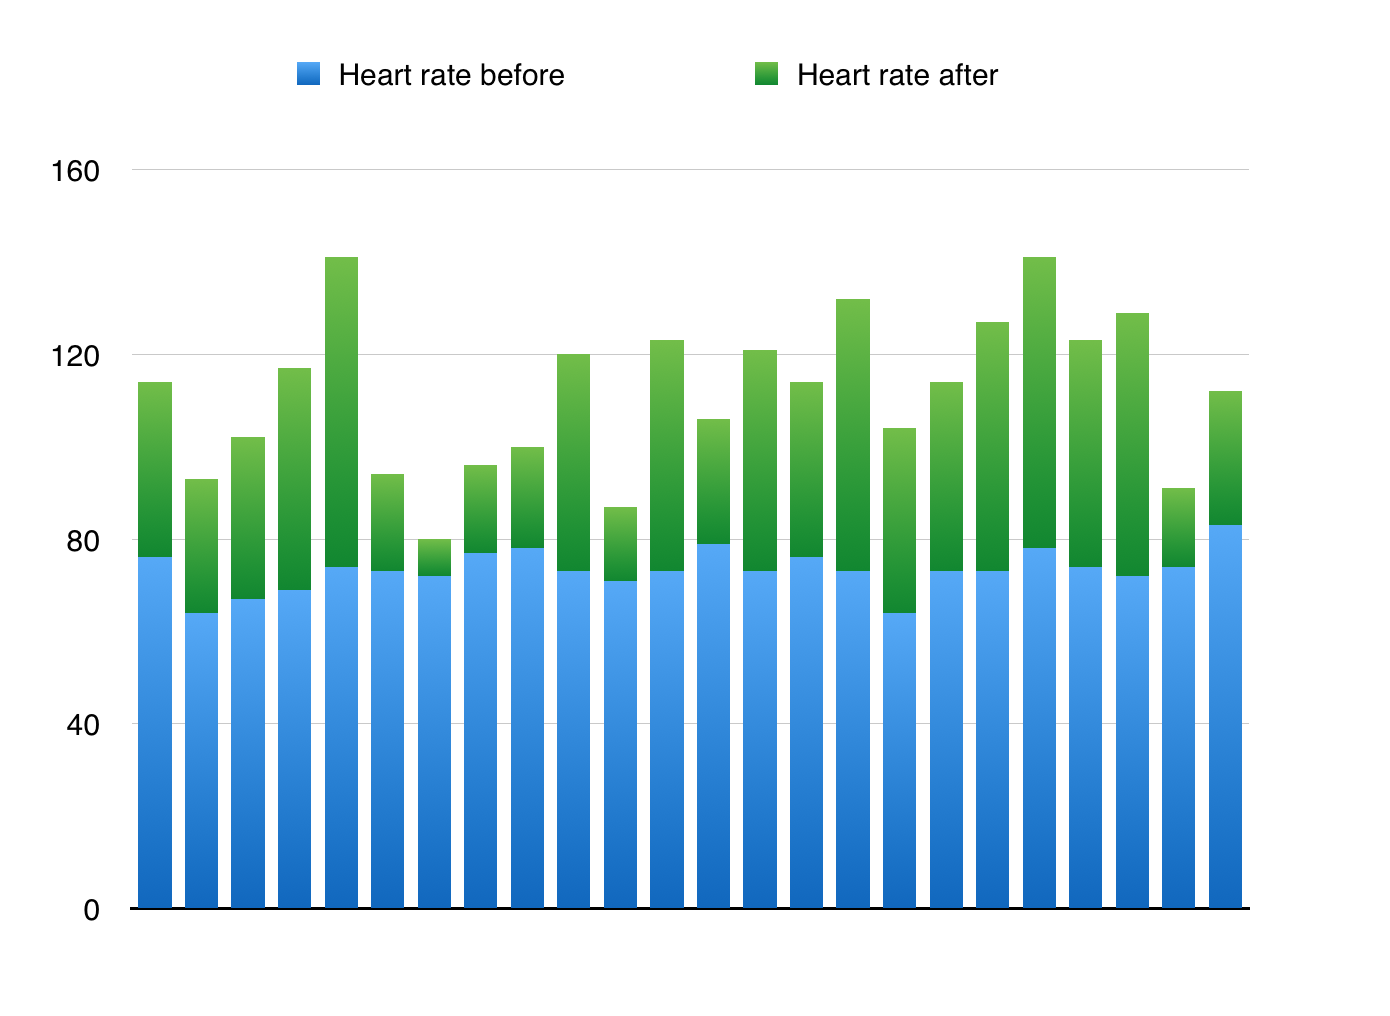
\includegraphics[scale=0.60]{../GFX/Resultsgraph.png}
	Figure 4.1: Graphical overview of the test results
\end{figure}

On average a player's heart rate increased with 52.9\% which is a very satisfied result with our requirement of a heart rate increase of 40\%.

\subsection{Feedback}
The children playing our game gave a lot of feedback to the game. As a spectator you could very clearly see that they were trying hard to remember the exercises especially in the higher rounds. What follows is a list of feedback given by the children.
\begin{itemize}
\item It is physically exhausting
\item You could clearly see when an exercise was done correctly by virtue of the green text on the screen with the points gained
\item It is hard to remember the order of exercises, especially when the exercises alternate very often
\item It is like using a Jump Rope (said by a girl who had many jumps)
\item Sometimes it was difficult to tell how high to jump and how low to squat in order for the game to register the exercise properly
\end{itemize}

\chapter{Conclusion \& Discussion}


\chapter{Further development}

\begin{thebibliography}{9}
\bibitem{Sundhedsstyrelsen}
  Sundhedsstyrelsen,
  \emph{Overv\ae gt}
  \url{http://sundhedsstyrelsen.dk/da/sundhed/overvaegt}

\bibitem{who-obesity}
	World Health Organization,
	\emph{Obesity}
	\url{http://www.who.int/topics/obesity/en/}
	
\bibitem{who-bmi}
	World Health Organization,
	\emph{BMI classification}
	\url{http://apps.who.int/bmi/index.jsp?introPage=intro_3.html}

\bibitem{consequences-obese}
	Ministeriet for Sundhed og Forebyggelse,
	\emph{Samfunds\o konomiske konsekvenser af sv\ae r overv\ae gt}
	\url{http://www.sum.dk/Aktuelt/Nyheder/Forebyggelse/2007/Maj/Samfundsoekonomiske_konsekvenser.aspx}

\end{thebibliography}


\chapter{Appendixes}

\end{document}
